\newpage
\section{Teilversuch 3: Messung der Eigenfrequenzen einer Luftsäule}
	Fehler bei Messung bzw. Steuerung der Frequenz $\Delta f_n = \SI{1}{\hertz}$\\
	Fehler bei Messung der Mikrofonspannung $\Delta U_\text{eff} = \SI{0.1}{\milli\volt}$

	\begin{center}
		\begin{tabular}{l *{11}{r}}
			\toprule
			$n$ & \num{0} & \num{1} & \num{2} & \num{3} & \num{4} & \num{5} & \num{6} & \num{7} & \num{8} & \num{9} & \num{10} \\
			\midrule
			$f_n / \si{\hertz}$ & \num{168} & \num{502} & \num{837} & \num{1171} & \num{1510} & \num{1843} & \num{2188} & \num{2541} & \num{2876} & \num{3210} & \num{3554} \\
			$U_\text{eff} / \si{\milli\volt}$ & \num{3.36} & \num{22.10} & \num{57.7} & \num{31.07} & \num{21.70} & \num{22.48} & \num{22.93} & \num{24.80} & \num{13.20} & \num{10.10} & \num{6.76} \\
			\bottomrule
		\end{tabular}
	\end{center}
	Laut Gleichung (6) der Anleitung hat $f_n$ und $n$ den folgenden Zusammenhang:
	\begin{equation}
		f_n = \frac{v}{4L^{*}} \pbrace{2n +1} = \left(\frac{v}{2L^{*}}\right)n + \frac{v}{4L^{*}} \equiv an+b
	\end{equation}
	Daraus folgt auch, dass die akustische Rohrlänge $L^{*}$ und der dazugehörige Fehler $\Delta L^{*}$ sich wie folgt brechnen lässt:
	\begin{align}
		L^{*} &= \frac{v}{2a} \label{eqn:akustiklange}\\
		\Delta L^{*} &= \gausserror{L^{*}}{v,a} \overset{\text{\scriptsize (AMW)}}{=} \frac{v}{2a}\sqrt{\pbrace{\frac{\Delta v}{v}}^2 + \pbrace{\frac{\Delta a}{a}}^2} \label{eqn:deltaakustiklange}
	\end{align}

	Die Daten wurden mit \gnuplot{} geplottet und eine Kurveanpassung wurde durchgeführt (Siehe Appendix \ref{appdx:gnuplotTV3}).
	\begin{figure}[H]
		\centering
		% GNUPLOT: LaTeX picture with Postscript
\begingroup
  \makeatletter
  \providecommand\color[2][]{%
    \GenericError{(gnuplot) \space\space\space\@spaces}{%
      Package color not loaded in conjunction with
      terminal option `colourtext'%
    }{See the gnuplot documentation for explanation.%
    }{Either use 'blacktext' in gnuplot or load the package
      color.sty in LaTeX.}%
    \renewcommand\color[2][]{}%
  }%
  \providecommand\includegraphics[2][]{%
    \GenericError{(gnuplot) \space\space\space\@spaces}{%
      Package graphicx or graphics not loaded%
    }{See the gnuplot documentation for explanation.%
    }{The gnuplot epslatex terminal needs graphicx.sty or graphics.sty.}%
    \renewcommand\includegraphics[2][]{}%
  }%
  \providecommand\rotatebox[2]{#2}%
  \@ifundefined{ifGPcolor}{%
    \newif\ifGPcolor
    \GPcolortrue
  }{}%
  \@ifundefined{ifGPblacktext}{%
    \newif\ifGPblacktext
    \GPblacktexttrue
  }{}%
  % define a \g@addto@macro without @ in the name:
  \let\gplgaddtomacro\g@addto@macro
  % define empty templates for all commands taking text:
  \gdef\gplbacktext{}%
  \gdef\gplfronttext{}%
  \makeatother
  \ifGPblacktext
    % no textcolor at all
    \def\colorrgb#1{}%
    \def\colorgray#1{}%
  \else
    % gray or color?
    \ifGPcolor
      \def\colorrgb#1{\color[rgb]{#1}}%
      \def\colorgray#1{\color[gray]{#1}}%
      \expandafter\def\csname LTw\endcsname{\color{white}}%
      \expandafter\def\csname LTb\endcsname{\color{black}}%
      \expandafter\def\csname LTa\endcsname{\color{black}}%
      \expandafter\def\csname LT0\endcsname{\color[rgb]{1,0,0}}%
      \expandafter\def\csname LT1\endcsname{\color[rgb]{0,1,0}}%
      \expandafter\def\csname LT2\endcsname{\color[rgb]{0,0,1}}%
      \expandafter\def\csname LT3\endcsname{\color[rgb]{1,0,1}}%
      \expandafter\def\csname LT4\endcsname{\color[rgb]{0,1,1}}%
      \expandafter\def\csname LT5\endcsname{\color[rgb]{1,1,0}}%
      \expandafter\def\csname LT6\endcsname{\color[rgb]{0,0,0}}%
      \expandafter\def\csname LT7\endcsname{\color[rgb]{1,0.3,0}}%
      \expandafter\def\csname LT8\endcsname{\color[rgb]{0.5,0.5,0.5}}%
    \else
      % gray
      \def\colorrgb#1{\color{black}}%
      \def\colorgray#1{\color[gray]{#1}}%
      \expandafter\def\csname LTw\endcsname{\color{white}}%
      \expandafter\def\csname LTb\endcsname{\color{black}}%
      \expandafter\def\csname LTa\endcsname{\color{black}}%
      \expandafter\def\csname LT0\endcsname{\color{black}}%
      \expandafter\def\csname LT1\endcsname{\color{black}}%
      \expandafter\def\csname LT2\endcsname{\color{black}}%
      \expandafter\def\csname LT3\endcsname{\color{black}}%
      \expandafter\def\csname LT4\endcsname{\color{black}}%
      \expandafter\def\csname LT5\endcsname{\color{black}}%
      \expandafter\def\csname LT6\endcsname{\color{black}}%
      \expandafter\def\csname LT7\endcsname{\color{black}}%
      \expandafter\def\csname LT8\endcsname{\color{black}}%
    \fi
  \fi
    \setlength{\unitlength}{0.0500bp}%
    \ifx\gptboxheight\undefined%
      \newlength{\gptboxheight}%
      \newlength{\gptboxwidth}%
      \newsavebox{\gptboxtext}%
    \fi%
    \setlength{\fboxrule}{0.5pt}%
    \setlength{\fboxsep}{1pt}%
\begin{picture}(7200.00,5040.00)%
    \gplgaddtomacro\gplbacktext{%
      \csname LTb\endcsname%%
      \put(814,704){\makebox(0,0)[r]{\strut{}$4,2$}}%
      \put(814,1112){\makebox(0,0)[r]{\strut{}$4,4$}}%
      \put(814,1521){\makebox(0,0)[r]{\strut{}$4,6$}}%
      \put(814,1929){\makebox(0,0)[r]{\strut{}$4,8$}}%
      \put(814,2337){\makebox(0,0)[r]{\strut{}$5$}}%
      \put(814,2746){\makebox(0,0)[r]{\strut{}$5,2$}}%
      \put(814,3154){\makebox(0,0)[r]{\strut{}$5,4$}}%
      \put(814,3562){\makebox(0,0)[r]{\strut{}$5,6$}}%
      \put(814,3971){\makebox(0,0)[r]{\strut{}$5,8$}}%
      \put(814,4379){\makebox(0,0)[r]{\strut{}$6$}}%
      \put(946,484){\makebox(0,0){\strut{}$-100$}}%
      \put(1478,484){\makebox(0,0){\strut{}$0$}}%
      \put(2011,484){\makebox(0,0){\strut{}$100$}}%
      \put(2543,484){\makebox(0,0){\strut{}$200$}}%
      \put(3076,484){\makebox(0,0){\strut{}$300$}}%
      \put(3608,484){\makebox(0,0){\strut{}$400$}}%
      \put(4141,484){\makebox(0,0){\strut{}$500$}}%
      \put(4673,484){\makebox(0,0){\strut{}$600$}}%
      \put(5206,484){\makebox(0,0){\strut{}$700$}}%
      \put(5738,484){\makebox(0,0){\strut{}$800$}}%
      \put(6271,484){\makebox(0,0){\strut{}$900$}}%
      \put(6803,484){\makebox(0,0){\strut{}$1000$}}%
    }%
    \gplgaddtomacro\gplfronttext{%
      \csname LTb\endcsname%%
      \put(209,2541){\rotatebox{-270}{\makebox(0,0){\strut{}$\ln \left[\left(h - h_\infty\right) / \si{\milli\meter}\right]$}}}%
      \put(3874,154){\makebox(0,0){\strut{}Zeit $t$ ($\si{\second}$)}}%
      \put(3874,4709){\makebox(0,0){\strut{}Wasserstand beim Kapilarviskosimeter im Verlauf der Zeit}}%
      \csname LTb\endcsname%%
      \put(5816,4206){\makebox(0,0)[r]{\strut{}$-0,00158x + 5,80951$}}%
      \csname LTb\endcsname%%
      \put(5816,3986){\makebox(0,0)[r]{\strut{}tv3.dat}}%
    }%
    \gplbacktext
    \put(0,0){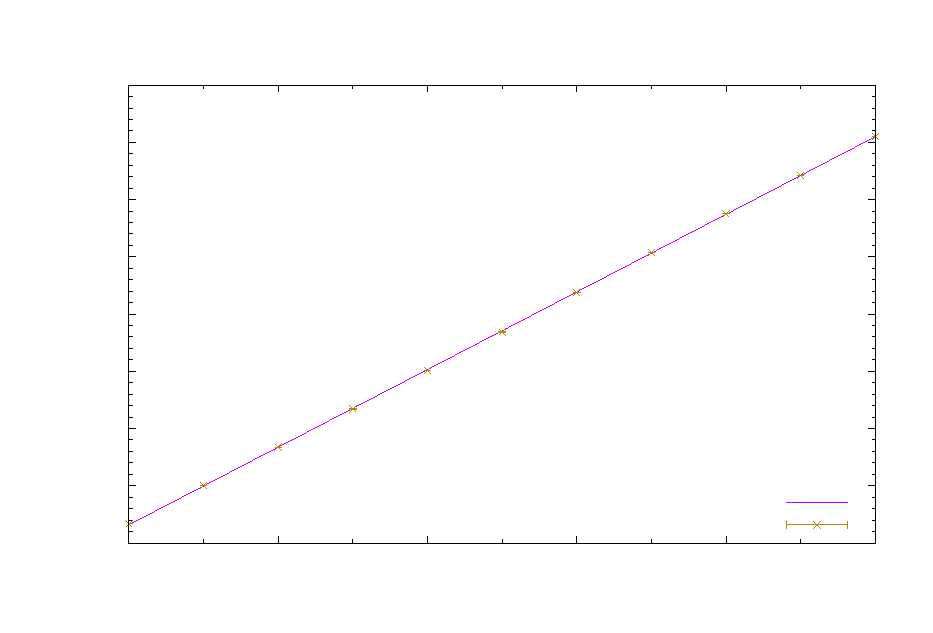
\includegraphics{tv3-plot}}%
    \gplfronttext
  \end{picture}%
\endgroup

		\caption{\centering Messung der Oberschwingungen des Rohres\captionbr $\chi^2_{\text{red}} = \num{46.698} > 1 \implies$ Schlechte Anpassung}
		\label{fig:tvthree-plot}
		\vspace{-1em}
	\end{figure}
	Die schlechte Anpassung kann vermutlich dadurch erklärt werden, dass die Bestimmung der Resonanzfrequenzen eher ungenau war, besonders bei der Steuerung des Sinus-Generator. In diesem Fall wurden aber die Messungenauigkeit der Frequenzen schon bei der Kurvenanpassung berücksichtigt. Es könnte dann sein, dass wir diese Ungenauigkeit wesentlich unterschätzt haben. 

	Als Endergebnis erhalten wir:
	\begin{center}
		\begin{tabular}{l r r}
			\toprule
			Variable & Rohausgabe & Gerundet \\
			\midrule
			$a$ & \SI{339,0636(6516)}{\hertz} & \SI{339.1(7)}{\hertz} \\
			$b$ & \SI{159.227(3855)}{\hertz} & \SI{159(4)}{\hertz} \\
			\bottomrule
		\end{tabular}
	\end{center}
	Wir benutzen in unserer Rechnungen die genauere Werte von $a$ und $\Delta a$ bzw. $v$ und $\Delta v$. In diesem Fall wurde für die Bestimmung der akustischen Rohrlänge aufgrund des geringeren Fehler $a$ statt $b$ gewählt, obwohl beide Werte theoretisch funktionieren könnten. 

	Mit der folgenden Werten:
    \begin{center}
        \begin{tabular}{lrl}
            \toprule
            Variable & Wert & Bedeutung \\
            \midrule
            $a$ & \SI{339,0636(6516)}{\hertz} & Gefundene Steigung der Gerade \\
            $v$ & \SI{344,424(1694)}{\meter\per\second} & Gefundene Schallgeschwindigkeit \\
            \bottomrule
        \end{tabular}
    \end{center}
    lässt sich mittels Gleichungen \eqref{eqn:akustiklange} und \eqref{eqn:deltaakustiklange} die akustische Rohrlänge $L^{*}$ und deren Fehler $\Delta L^{*}$ bestimmen:
    \begin{align}
    	L^{*} &= \frac{\SI{344,424}{\meter\per\second}}{2\pbrace{\SI{339,0636}{\hertz}}} = \SI{0,507905}{\meter} \sigfig{6} \\
    	\Delta L^{*} &= \frac{\SI{344,424}{\meter\per\second}}{2\pbrace{\SI{339,0636}{\hertz}}} \sqrt{\pbrace{\frac{\SI{1.694}{\meter\per\second}}{\SI{344,424}{\meter\per\second}}}^2 + \pbrace{\frac{\SI{0.6516}{\hertz}}{\SI{339,0636}{\hertz}}}^2} \notag \\
    	&= \SI{2,682e-3}{\meter} \sigfig{4}
    \end{align}
    Daraus folgt, dass die akustische Rohrlänge $L^{*} = \SI{0,5079(27)}{\meter} = \SI{507.9(27)}{\milli\meter}$.

    Im Vergleich dazu ist die gemessene Rohrlänge $L = \SI{50.0(1)}{\centi\meter} = \SI{500(1)}{\milli\meter}$. Das Fehlerintervall der beiden Werten überschneiden sich miteinander nicht, also ist $L^{*} > L$, was zu erwarten ist. 